\section{Comparative Analysis of Building Modeling Software}

In this section, popular solutions in the market for modeling buildings will be analyzed,
highlighting each solution's strengths and weaknesses.
A table is then presented, summarizing each solution by its most relevant features.
This section ends with the discussion regarding the better features of the analyzed software.

\subsection{AutoCAD}
AutoCAD \cite{SITE-AUTOCAD} is the \emph{de facto} standard software for architecture designs.
It has a steep learning curve (Fig.\ref{FIG-AUTOCAD}) but is nevertheless
learned all over the world.
One of its formats, DXF, is widely supported by 3D modeling software.
AutoCAD features a powerful language, AutoLisp, which allows advanced users to create scripts for
automating any aspect available in the interface.
This program favors 2D drawing and modeling over real 3D concepts,
but a skillful operator can create every shape necessary to an architectural scenario.
Internally AutoCAD doesn't support interactive previewing of the created designs.
It renders using the powerful Mental Ray\nocite{SITE-MENTAL} engine.
Animations can be made using camera paths.

There are hundreds of commercial plug-ins extending the capabilities of AutoCAD in a multitude of features.

\begin{figure}[!ht]
    \centering
    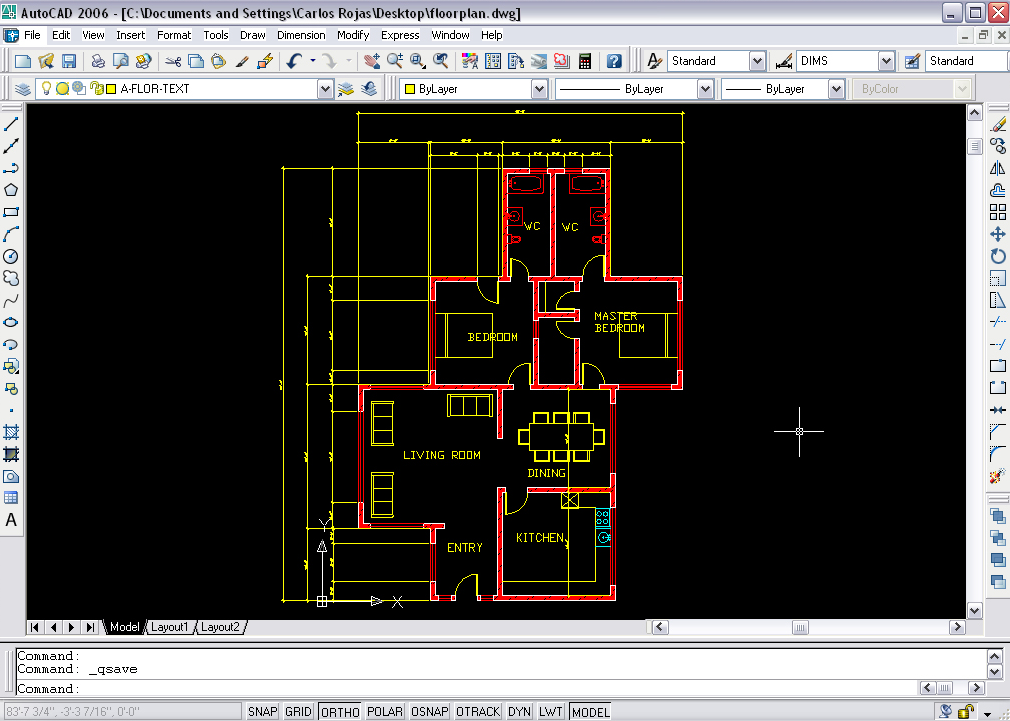
\includegraphics[width=9cm]{gfx/autocad-1.png}
    \caption{AutoCAD: A typical layout of a floor plan.}
    \label{FIG-AUTOCAD}
\end{figure}

\subsection{ArchiCAD}
GraphiCad's ArchiCAD \cite{SITE-ARCHICAD} aims at conquering the new generation of architects who haven't been exposed to AutoCAD.
It offers pre-made views and document templates for every architectural driven need.
It is by definition a 3D CAD program and it is praised by architects for its easy 3D
manipulation capabilities (Fig.\ref{FIG-ARCHICAD}).

The program features templates for common architectural elements.
ArchiCAD has navigation capabilities too, allowing first person perspective navigation of the model.
Its workflow is thought out to make it easy for an architect to do the most common tasks,
making it a friendlier alternative when compared to AutoCAD.
It lacks the expressive power to do about 10\% uncommon tasks though.
There's a Software Development Kit for ArchiCAD plug-in creation.

\begin{figure}[!ht]
    \centering
    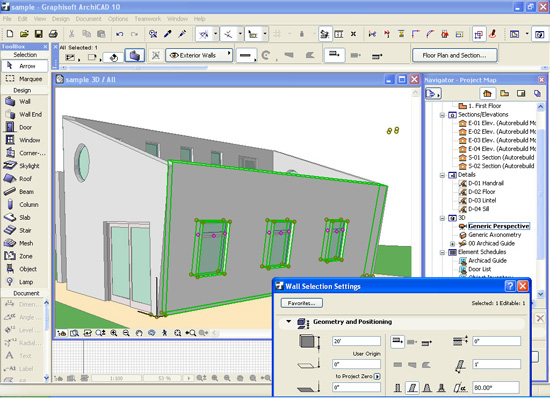
\includegraphics[width=9cm]{gfx/archicad-1.png}
    \caption{ArchiCAD: Notice basic selection and template properties editing in the 3D view.}
    \label{FIG-ARCHICAD}
\end{figure}

\subsection{Revit Building}
Revit Building \cite{SITE-REVIT} is another Autodesk product.
Unlike AutoCAD, which spans its use to other areas such as mechanical engineering,
Revit Building was explicitly thought out for architectural design.

It works completely in 3D and has native templates for doors, windows, roofs, etc.
Common constraints are detected. Thick walls can be drawn as lines and solids can
be cut as floors (compare the top-left and bottom right views in Fig.\ref{FIG-REVIT}).

Revit Building features powerful templates for complex tasks such as roof design.
It has a simple raytracing and radiosity engine.
Cameras can be placed for view rendering but not animation.

Being a system for the professional segment, it has a smoother learning curve than
AutoCAD and provides tools that allow successful modeling of complex buildings,
even for enthusiasts, a quality not held by AutoCAD.

\begin{figure}[!ht]
    \centering
    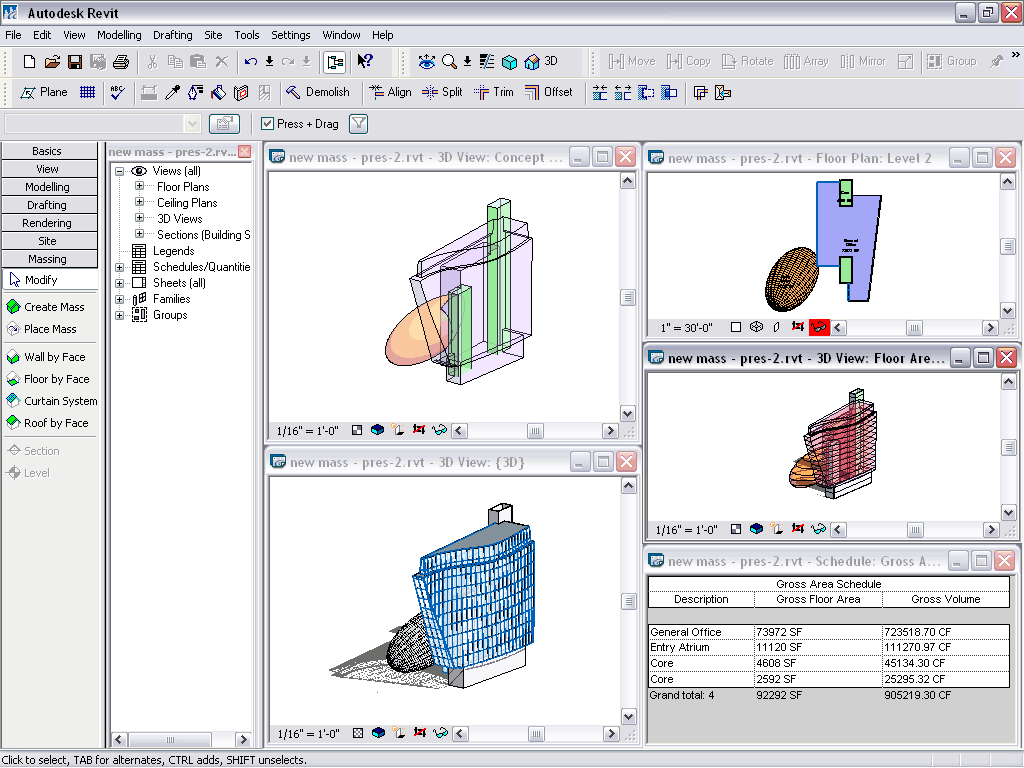
\includegraphics[width=9cm]{gfx/revit-1.png}
    \caption{Revit Building: Solid shapes can be combined with boolean operations and converted into buildings.}
    \label{FIG-REVIT}
\end{figure}

\subsection{SketchUp}
Google SketchUp \cite{SITE-SKETCHUP} is a friendly program for the novice 3D modeler.
It features a simple toolbar interface with 1 viewport and most of its tools are basic.
One is still able to achieve acceptable results with it.
Its learning curve is good.
Its engine is based on drawing lines on top of lines,
already created surfaces or a construction plane.
It detects the most common geometry restrictions (such as midpoint and perpendicularity).
It features an online repository of models, allowing importing of objects such as
furniture, trees, props or well known buildings by browsing and selection.
Strange results occur when handling awkward angles
or several lines are the vicinity of the mouse.
Curve manipulation and generation of surfaces is nonexistent.
SketchUp allows plug-in design using the Ruby language.

Another bonus from being part of the Google software library, SketchUp features import/export capabilities with Google Earth \cite{SITE-EARTH}.
This allows capturing a patch of land from Google Earth to SketchUp, design a building there and export the result
back with its new contents to the map.
A great feature SketchUp has is realtime shadows (see figure \ref{FIG-SKETCHUP})
-- since there's only one viewport, shadows are crucial to give the user a sense of depth to a scene.

It renders configurable non-photorealistic lines and fillings and allows
interpolating between camera instances in order to obtain simple animations.
It provides importing capabilities from the most common 3D formats.
The professional version of the program allows exporting to common 3D architectural formats too.


\begin{figure}[!ht]
    \centering
    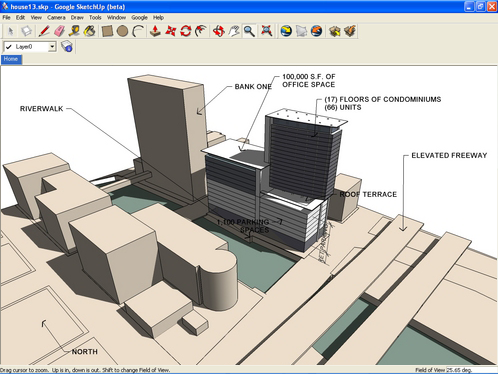
\includegraphics[width=9cm]{gfx/sketchup-1.png}
    \caption{SketchUp: Basic shape extrusions. Notice the shadows in the viewport.}
    \label{FIG-SKETCHUP}
\end{figure}

\newpage

\subsection{Comparison Table of Available Solutions}
\begin{table}[!ht]
  \centering
	\begin{tabular}{|c|c|c|c|c|}
		\hline
		\backslashbox{Features}{Solutions}		& AutoCAD		& ArchiCAD	& Revit Building	& SketchUp	\\
		\hline
		Design in 2D						&		\GdA		&		\GdB		&				\GdB			&		\GdC		\\
		\hline
		Design in 3D						&		\GdD		&		\GdC		&				\GdB			&		\GdB		\\
		\hline
		Architectural Templates	&		\GdD \footnotemark		&		\GdB		&				\GdA			&		\GdE		\\
		\hline
		Supported Formats				&		\GdC		&		\GdC		&				\GdB			&		\GdD / \GdB \footnotemark\\
		\hline
		Interactive Modes				&		\GdE		&		\GdB		&				\GdC 			&		\GdE		\\
		\hline
		Rendering Capabilities	&		\GdB		&		\GdB		&				\GdC			&		\GdD		\\
		\hline
		Extensibility						&		\GdB		&		\GdC		&				\GdD			&		\GdC		\\
		\hline
	\end{tabular}
	%\caption{Different solutions in the market compared.}
	%\label{TB-COMP-SOL}
\end{table}
\footnotetext[1]{without any additional plug-in}
\footnotetext{SketchUp exporting capabilities depend on using free or commercial version}

\vspace{-0.5cm}
\begin{table}[!ht]
  \centering
	\begin{tabular}{|p{1.1cm}|p{1.1cm}|p{1.1cm}|p{1.1cm}|p{1.1cm}|}
		\hline
		\scriptsize{very bad}	& \scriptsize{bad}			& \scriptsize{average}	& \scriptsize{good}		& \scriptsize{very good}	\\
		\hline
		\GdE									&	\GdD									&	\GdC									&	\GdB								&	\GdA			\\
		\hline
	\end{tabular}
	%\caption{Legend of Table \ref{TB-COMP-SOL}}
  %\label{TB-COMP-SOL-LEGEND}
  \caption{Different solutions in the market compared.}
  \label{TB-COMP-SOL}
\end{table}

\subsection{Discussion}
AutoCAD makes use of a well established workflow which takes time to master.
There's a way of modeling everything architecturally speaking, though many
tasks require expert training to be done.
Since its a general purpose package, supporting other areas such as mechanical engineering,
AutoCAD doesn't come with architectural templates,
a very helpful feature available in both ArchiCAD and Revit Building.

Revit Building is Autodesk's vision of an easy to master,
yet powerful system for architectural design.
Revit Building and ArchiCAD are the most similar of the compared systems.
Revit Building has better modeling features while ArchiCAD has many document templates
ready for extracting bureaucratic papers out of the architect's workflow.

SketchUp is the most amateur of the analyzed systems.
It offers limited geometrical operations and doesn't have a real template library.
It tries to overcome that limitation by offering a large online repository of models.
SketchUp's best qualities are its learning curve and its Google Earth connection.

It would be of great use if other programs were granted permission to get geographical
data (both height maps and texture maps) from Google Earth.
This would offer an important head-start for an architect in designing a building that
smoothly blends in its surroundings.
Since this software was acquired by Google and associated with Google Earth,
a large SketchUp use base is taking shape.

\TODO{BETTER STUFF FROM EACH SW FOR PROJECT?}